
In this chapter we address the \ac{HRI} systems, the \ac{Wiimote}, the kinect, and the iCub related work.

\section{\acf{HRI}}  %\ref{sect:\acf{HRI}}

	A robot autonomy level can be measured by the percentage of time that a robot does not need intervention to realize a task \cite{hri:Yanco04classifyinghuman-robot}. Nowadays robots are still not completely prepared to be autonomous and understand our language, but they have become useful in many tasks as helpers \cite{hri:robonaut}. \ac{HRI} is responsible for the way of ``communicating'' with a robot and control how it may help us in a task.

	The problem of natural movements in robots as been approached in several different forms, the solution is divided into two parts: the users interaction and the robot response. Relating both parts there is the gesture that it is as important as the way we do the gesture \cite{hri:Ou:2010:MCG:1734454.1734563} so that we can be comprehended, so it is important that a social robot such as the iCub is able not only to repeat a gesture, but also to reproduce it in a natural way, retrieving characteristics from the users interaction.

	In the iCub robot case there have recently been presented some works in which a user controls the robot by making pressure on its artificial skin \cite{hri:Sauser:2011:LIL:1957656.1957798}, or a robot movement can be programmed by a user that pushes the robot parts. This type of interaction is particularly useful when learning by demonstration, because the information from some interaction devices may be easily depured and sent to the robot. Several works on this subject already use one of these kinds of interaction \cite{hri:5480475}. From another perspective to face this ``communication'' problem there have been several approaches. Many use teleoperation \cite{hri:1512452} where the user and the robot do not have any contact, not even needing to be in the same room.

	In the last few years there were several gaming interfaces, introduce by gaming companies, that have contributed for the development of the \ac{HCI} and from which \ac{HRI} has taken advantage. Game controllers have been compared by other works \cite{hri:eu}, and considered as suitable for motion capture, with these controllers it is possible to build cheap and robust interaction systems, and that are already known by a large group of users. Two very recent, but very sophisticated, examples of good gaming controllers are the \ac{Wiimote} and the Xbox Kinect, these have made possible for developers to access cheap accelerometers, gyroscopes and depth cameras. From this accessibility there have been appearing new possibilities for \ac{HRI} systems.
	
	

%|-----------------------------------------|
%|------------- WIIMOTE PART --------------|
%|-----------------------------------------|

\section{Wii remote} %\ref{sect:\acf{Wiimote}}

The \ac{Wiimote} is the main controller for the Nintendo Wii Gaming console. This gaming remote control is differentiated from its competitors due to its motion sensing capability, which allow the user to interact through it with gestures.

Also the \ac{Wiimote} allows for expansion attachments to be used and augment its capabilities. This expansions range from the addition of gyroscopes, to game specific hardware as a gamepad guitar, or steering wheel. In figure \ref{fig:wiimotemotionplus} it is shown a \ac{Wiimote} with a Motion Plus extension attached which is highlighted by a blue circle.

 	\begin{figure}[htb]
	\begin{center}
	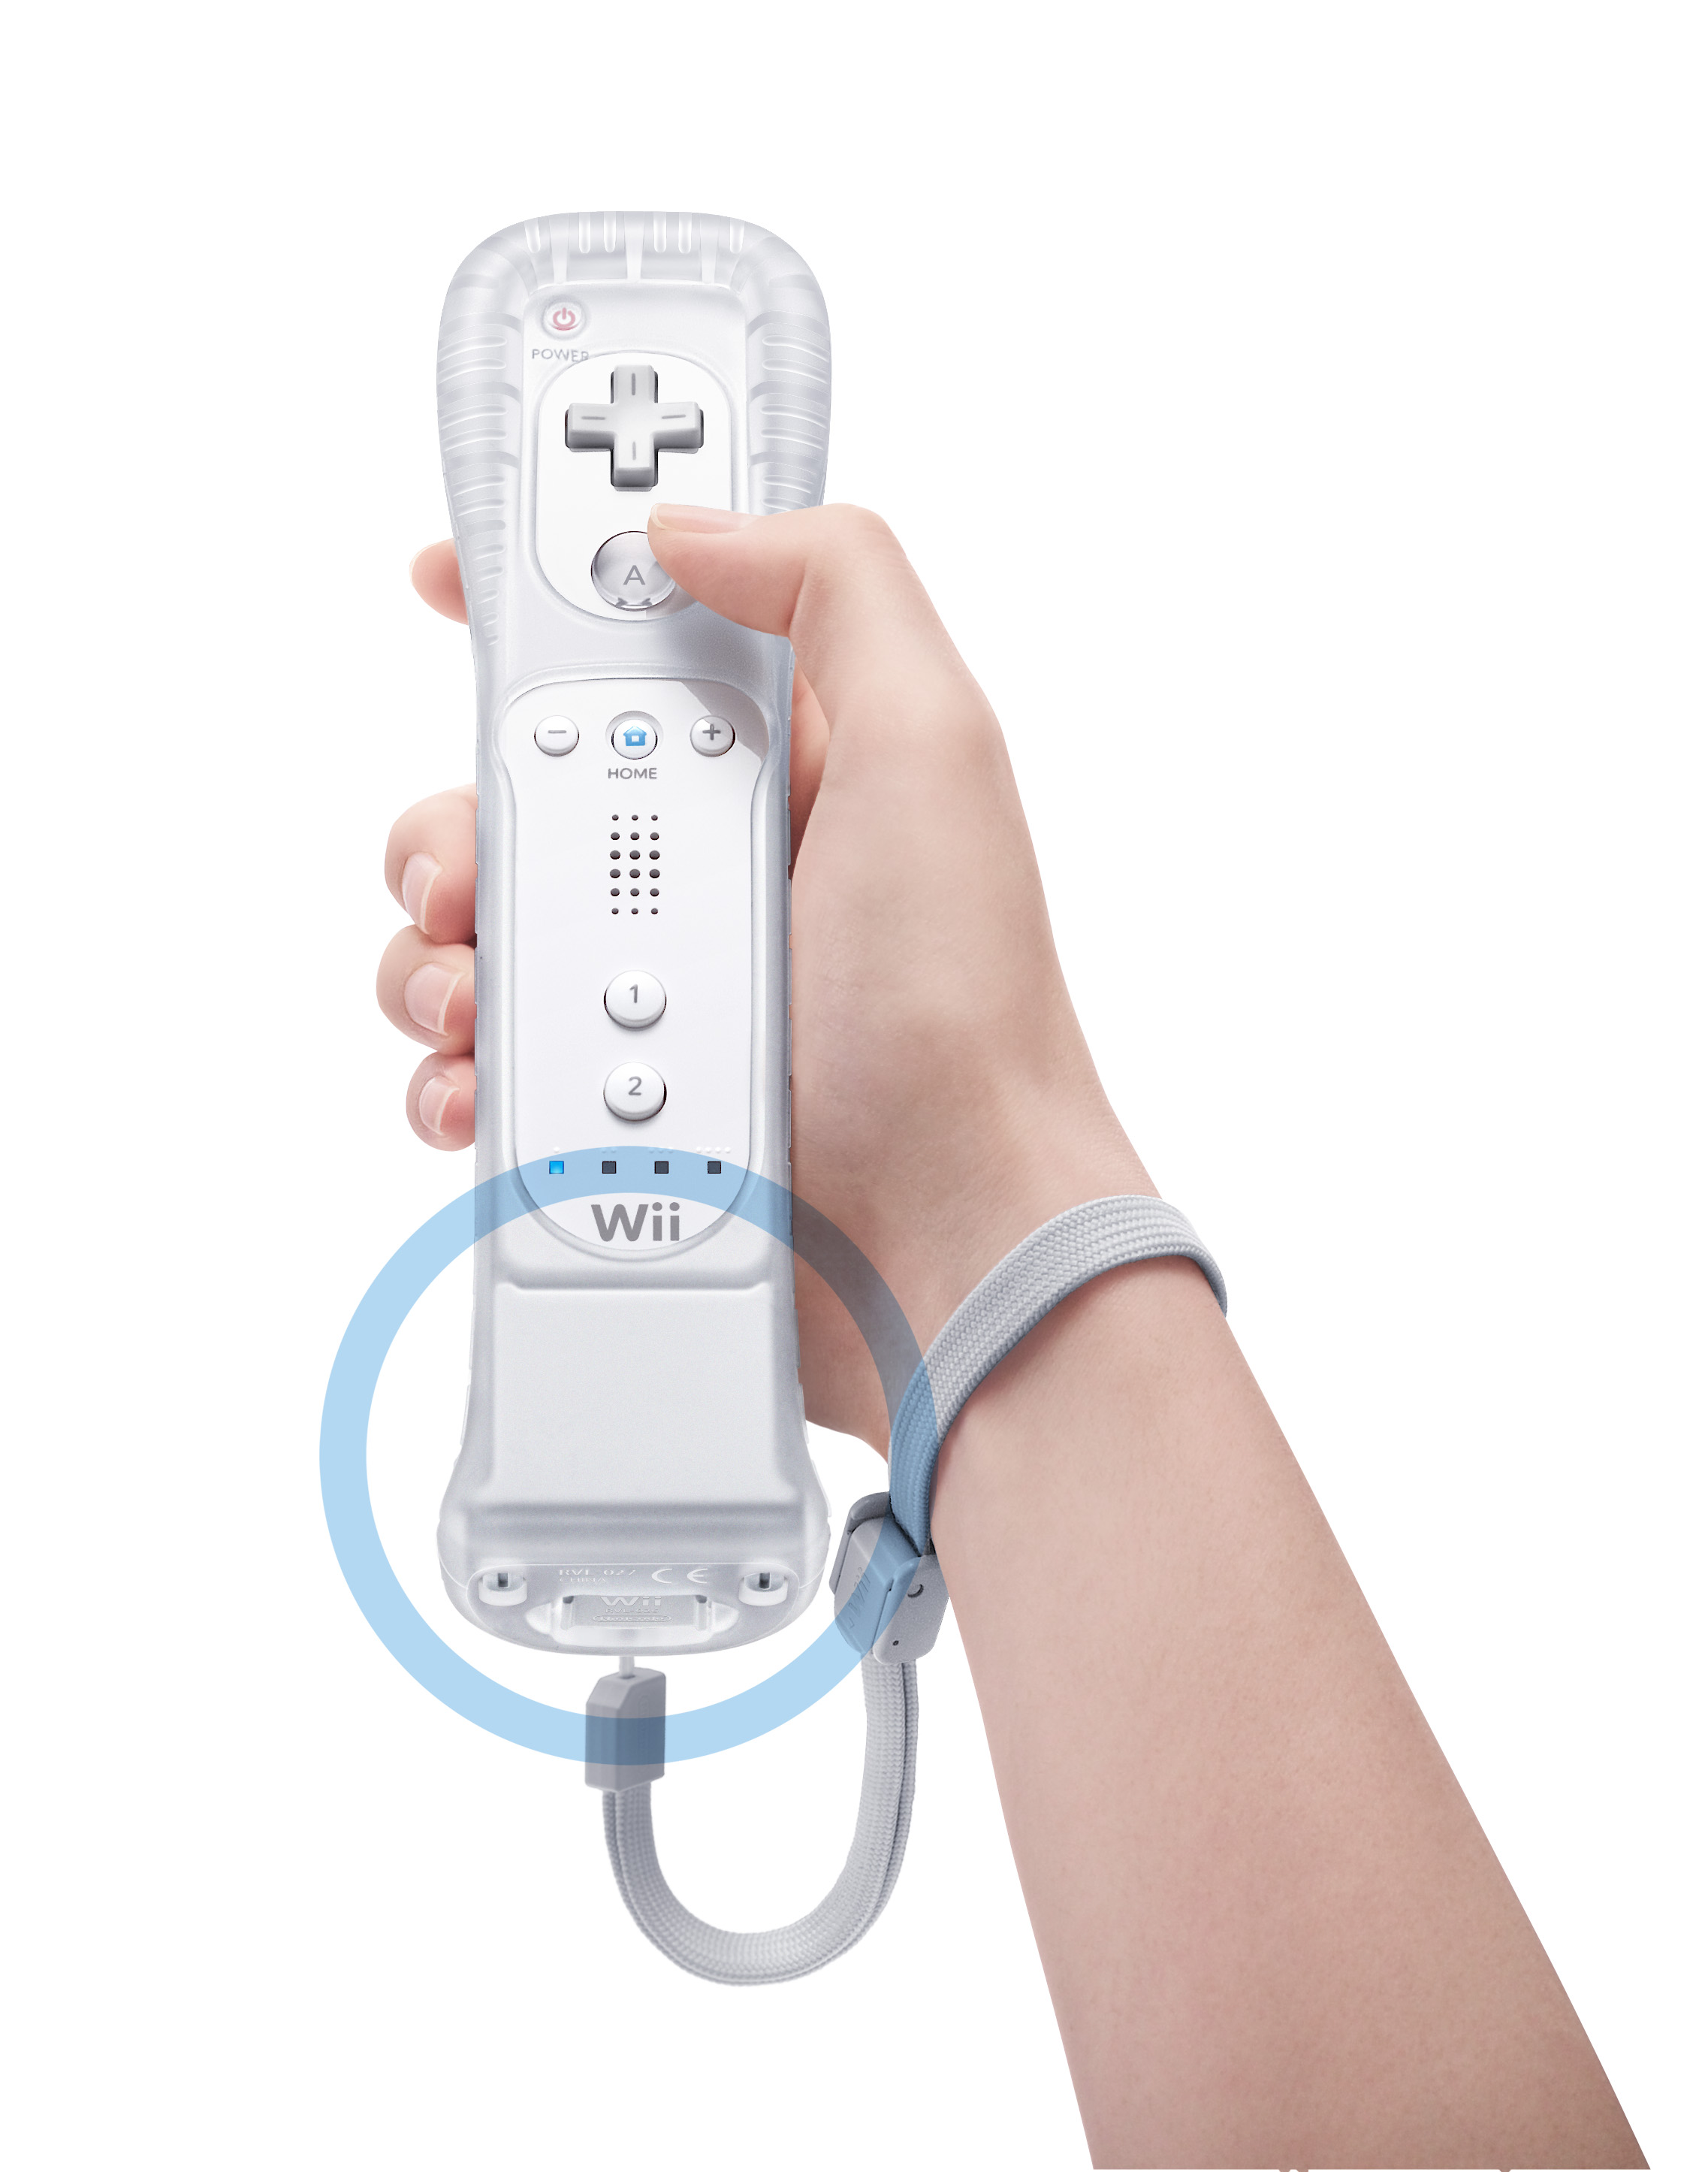
\includegraphics[height=72mm]{wiimotemotionplus.jpg}
	\end{center}
	\caption[Wiimote with the Motion Plus extension attached]{Wiimote with the Motion Plus extension attached.} 
	\label{fig:wiimotemotionplus}
	\end{figure}


The \ac{Wiimote} was revealed at the Tokyo Game Show on October 14, 2005. Due to its unique features at the time, it gained significant attention from hackers for non Wii or gaming purposes \cite{wiki:wiimote}.

There are now several other interesting interaction devices, with similar features, some of which were revealed during the development of this work, as the PlayStation 2 (PS2) EyeToy\footnote{\url{http://en.wikipedia.org/wiki/EyeToy}}, the PlayStation 3's (PS3) Eye\footnote{\url{http://en.wikipedia.org/wiki/PlayStation_Eye}}, the PS3 Move\footnote{\url{http://en.wikipedia.org/wiki/PlayStation_Move}}, or the Microsoft Kinect\footnote{\url{http://en.wikipedia.org/wiki/Kinect}}.

\subsection{Specifications}

Although the \ac{Wiimote} official specifications are unpublished, the global hacking community has collectively reverse-engineered a significant portion of the technical information regarding its internal workings. Much of this work has been collected from online wikis at \url{http://wiili.org} and \url{http://wiibrew.org}. Johnny Chung Lee has contributed with a specification as a result of the wikis information \cite{10.1109/MPRV.2008.53}.

The \ac{Wiimote} has an \ac{IR} Camera, a Accelerometer, twelve push-buttons, a vibration motor, a speaker, a bluetooth chip, internal flash memory and an expansion port. To be used with the \ac{Wiimote} there is a ``Sensor Bar'' with \ac{IR} emitters, and the expansion port allows the connection of other devices to expand functionality.

The \ac{IR} Camera sensor has a \ac{MOT} engine that allows high-speed, high-resolution \ac{IR} sources tracking. There can be a maximum of four \ac{IR} light sources, that are mapped in a 1024x768 pixel space at 100Hz refresh rate, according to position and intensity of each \ac{IR} light source.

The Accelerometer was manufactured by Analog Devices, the one embedded in the \ac{Wiimote} is model ADXL330. This model is a 3-axis linear accelerometer, with a sensitivity range of +/-3g (gravitational acceleration), and returns 8 bits of information per axis at a 100Hz update rate.

There are 12 Buttons arranged in a symmetrical way so that the remote can be held either with the left or right hand. On the bottom of the \ac{Wiimote} there is one trigger-like button, at the top there are four directional buttons (a typical \ac{DPad}), a plus and minus buttons, a home button, one A button, two number buttons (one and two), and inside the battery case there is a synchronize button. The trigger-like button is used with the index finger, all the others are best accessed with the thumb, except the synchronization button which is hidden inside the battery case. In the appendix \ref{appendix:Wiimote manual} are presented the pages of the official Wii console manual, that show and identify all the \ac{Wiimote} buttons.

The Vibration Motor is similar to the ones found in mobile phones, and can only be set ON and OFF.

The four \acp{LED} at the lower part of the \ac{Wiimote} can be individually addressed and only have a binary state.

The Speaker in the \acp{Wiimote} center can play audio data with 4-bit, 4KHz sound, similar to telephone quality. This is the part of the \ac{Wiimote} about which there is less information.

The communication is made through a Bluetooth connection. This system uses a Broadcom 2042 chip, which was designed for devices that conform to the Bluetooth \ac{HID} Standard. 

The \ac{Wiimote} has a Internal Flash Memory of approximately 5.5KB, that is used for the device settings, maintaining output and storing data.

The Expansion Port is on the bottom part of the \ac{Wiimote} and it is a proprietary six-pin connector. This connector is used to communicate with a power extension, and with extensions such as the Nunchuck or the \ac{MP}. The port provides a 3.3V power and 400Khz of \ac{I2C} serial communication to which a microcontroller can easily provide a Bluetooth-to-\ac{I2C} bridge.

To operate the \ac{Wiimote} needs two AA batteries and has an operating time of 20 to 40 hours. The battery level can be checked trough an 8-bit value.

\subsection{\acf{MP}}

	The \ac{MP} was released in June 2009 \cite{wiki:wiimotionplus} as an extension for the \ac{Wiimote}. The \ac{MP} makes the \ac{Wiimote} interaction more precise, by measuring the rotation change applied to the remote.
 
	Inside the \ac{MP} there is a dual-axis gyro by InvenSense, the IDG-600(pitch and roll), and a single-axis gyro by EPSON TOYOCOM labeled X3500W (yaw). These two gyroscopes allow to measure the rate of rotation along all 3-axes of X (pitch), Y (roll), and Z (yaw), as shown in figure \ref{fig:wiimoteAxis}. Specifications of the X3500W are currently unknown, but in the Invense website the IDG-600 specifications can be found \footnote{\url{http://invensense.com/mems/gaming.html}}:
\begin{itemize}
\item Highest range to measure fast controller motions up to $\pm$2.000�/sec full scale range.
\item Two separate outputs per axis for standard and high sensitivity, reduces system cost by permitting use of lower resolution analog-to-digital converters (ADC). Depending on the speed detected, the sensitivity changes.
\item IDG-650 has an integrated single-chip in-plane design with superior X/Y cross-axis alignment. ISZ-650 single-axis (Z) gyro complements the IDG-650 dual-axis (X/Y) gyro for a 3-axis gyro solution where all sensors mount in-plane with other system electronics.
\item Superior vibration rejection by design.
\item Highest shock resistance at 10,000g.
\item Auto-zero function minimizes bias drift.
\item World smallest dual-axis gyro form factor at 4x5x1.2mm.
\item Nasiri-Fabrication platform delivers inherent size, performance and cost advantages unattainable with competing fabrication processes.
\end{itemize}

\subsection{\ac{Wiimote} interaction}

With the \ac{Wiimote} introduction in the mass market there was a high interest of the scientific community in using this device for its own research. As cited by many works \cite{springerlink:robotontheleash,wiimote:azmi2009wiimote} the \ac{Wiimote} has the advantage of being inexpensive and can be used as a tangible natural interaction device.

The \ac{Wiimote} is considered as a spatial convenient device \cite{wiimote:10.1109/MCG.2009.109}, because it respects three main characteristics: provides spatial data, has sensors and emitters and it is inexpensive and durable. Having these characteristics into consideration, the \ac{Wiimote} is defined as a useful 3D User Interface.

The works that use this device range from motion control systems \cite{wiimote:lowcostmultipledegrees}, to robotic user interface \cite{wiimote:bascetincelik2009wiirobot}, or even art projects \cite{WiiArts:Lee:2008:WCC:1347390.1347400}. The flexibility and ease of use has been presented as a efficient interface for robotic control on several works \cite{springerlink:robotontheleash,wiimote:bascetincelik2009wiirobot,wiimote:Guo:2008:EUT:1357054.1357076}. These works typically compare traditional interface methods with the \ac{Wiimote} interface, where the accelerometer and \ac{IR} camera are used to control a robot or a 3D environment.

The accelerometer in the \ac{Wiimote} allows to independently get the current orientation of the remote, and the amount of force applied to the remote in respect to the gravity \cite{wiimote:Guo:2008:EUT:1357054.1357076}. Examples of this system are described in works that try through this way to capture human motion models \cite{wiimote:humanmotionmomodels}, interface with robots \cite{wiimote:Guo:2008:EUT:1357054.1357076} or assist in rehabilitation therapy \cite{wiimote:4625137}. One of the main challenges with the usage of the accelerometers in the \ac{Wiimote} is the noise that they produce. To avoid this problem a Kalman filter is often used. This filters out the noise by observing the noisy data retrieved over time and calculating estimates of the true values of that data. Also the accelerometer can not retrieve the orientation of the \ac{Wiimote} with all the degrees of freedom, because a rotation made around the axis of gravity is not detected. This limits the \ac{Wiimote} to gesture detection, and does not really do motion tracking except in very controlled situations.

To overcome this the \ac{IR} Camera can detect up to four different \ac{IR} sources, with that data it is possible to understand the \ac{Wiimote} position by triangulation, with the ``sensor bar'' serving as reference point. Although the typical usage of this feature is with the \ac{Wiimote}/camera in the hand, a lot of the studied systems keep the IR Camera still and have a moving \ac{IR} light source that is detected. This allows the interface developed to be less intrusive since the user only needs to have an invisible light (\ac{IR}) source, the main disadvantage in this solution is the spatial limitation of the camera angle. Following the fixed camera idea, there were experiments made with two \acp{Wiimote} \cite{wiimote:murgia2008low,wiimote:Scherfgen:2009:TUM:1639601.1639620}, this way it is possible to get a better definition, the opposite technique as also been tested using two light sources, in distinct places, to make the triangulation \cite{wiimote:azmi2009wiimote}.

The \ac{MP} was sold as a \ac{Wiimote} extension although nowadays its gyroscope is shipped as a part of the \ac{Wiimote} device. The introduction of this gyroscope allows the \ac{Wiimote} to have more precise data about the angular changes made. The merge between the accelerometer data and the gyroscope data allows for a more accurate orientation tracking
 \cite{wiimote:10.1109/MCG.2009.109,wiimote:dufourdevelopment}. Although the \ac{MP} adds accuracy, it obliges the user to make a calibration before using it, which might not be so straightforward.
 
%|-----------------------------------------|
%|-------------- KINECT PART --------------|
%|-----------------------------------------|


\section{Kinect} %\ref{sect:Kinect}

 The Kinect for the Xbox 360 console from Microsoft\footnote{\url{http://www.xbox.com/en-US/Kinect/}}, shown in figure \ref{fig:kinectsensor}, is a webcam style device add-on that allows a controller free gaming interaction. The Kinect was released in Europe  on November 10, 2010\footnote{\url{http://en.wikipedia.org/wiki/Kinect}}, so it is still a quite novel device. Although the Kinect is still the only one of its kind existing, with such a low price, Microsoft competitors are beginning to emerge, as it is possible to see by the unreleased but rumored Asus Wavi Xtion Motion\footnote{\url{http://tinyurl.com/4l5lu5a}}, which copies much of the Kinect functionality.
 
 	\begin{figure}[htb]
	\begin{center}
	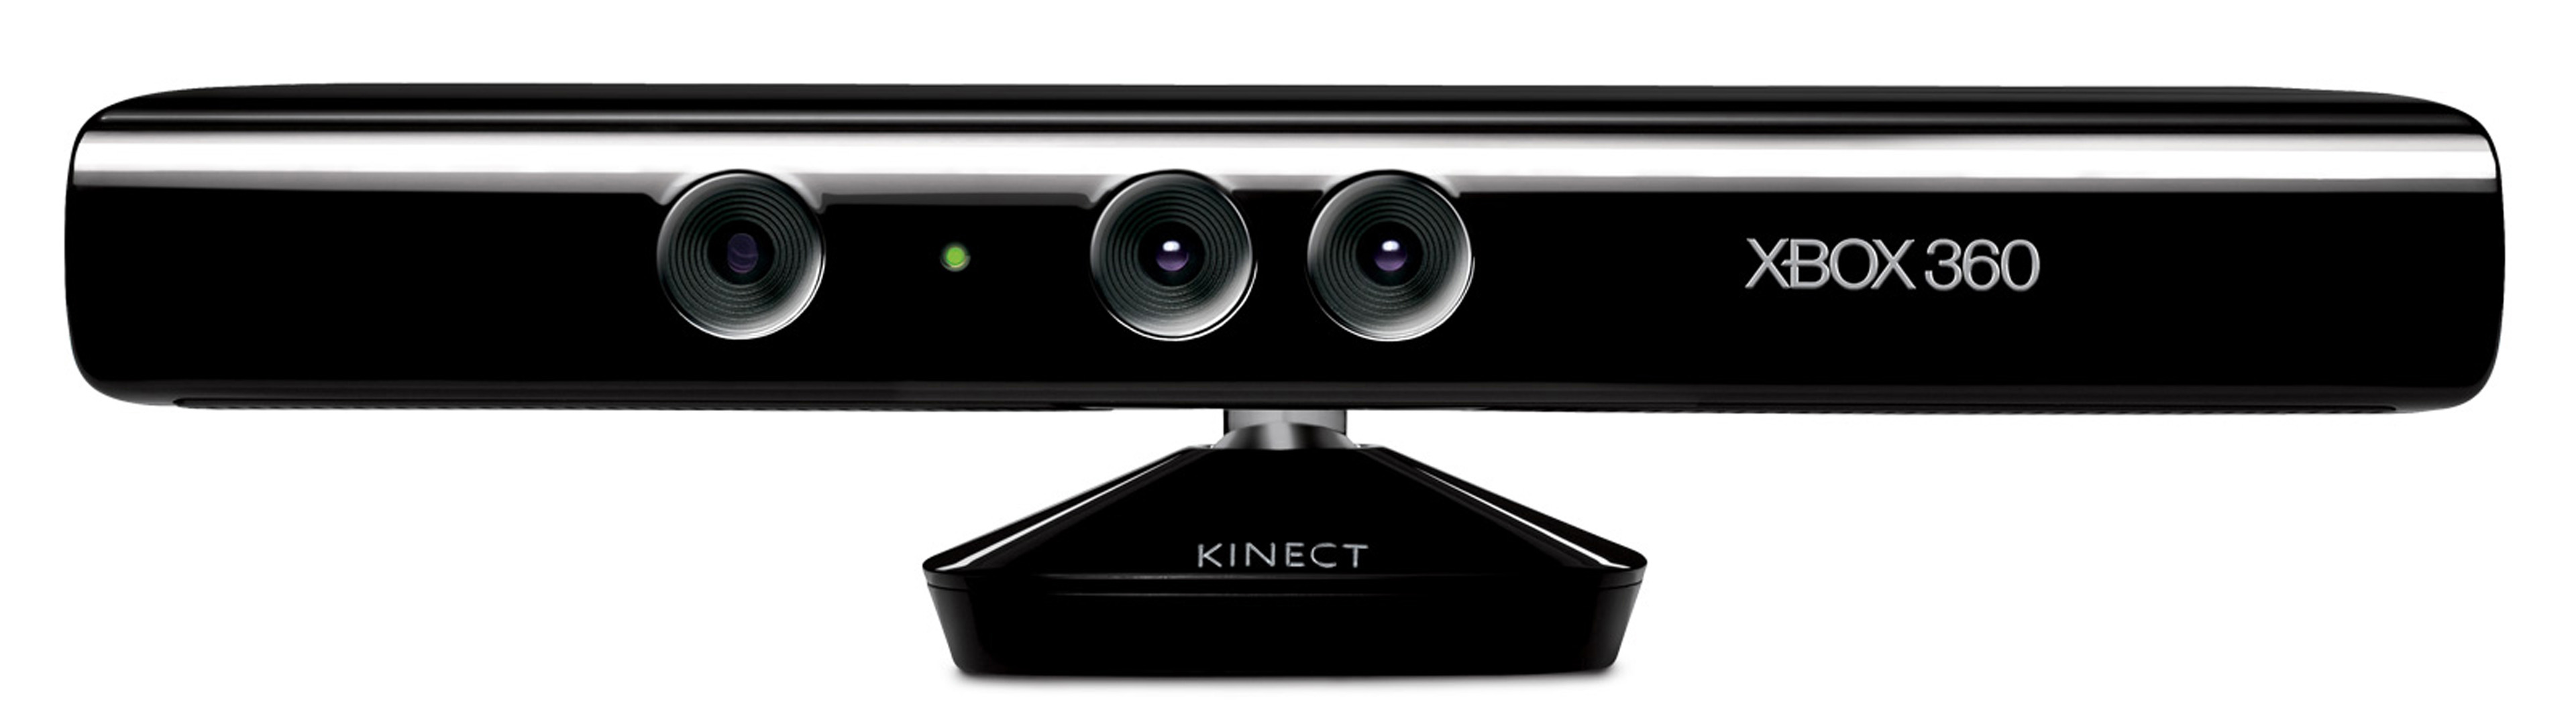
\includegraphics[width=72mm]{kinectsensor.jpg}
	\end{center}
	\caption[Microsoft Kinect sensor]{Microsoft Kinect sensor.} 
	\label{fig:kinectsensor}
	\end{figure}
 
 	The technology  used by the Kinect to produce its result is quite old, but the algorithms that it uses for skeleton detection and user tracking are the ones being presented as innovations in the gaming world. The systems that are used with this sensor allow to control games using the user body without any type of controller in the user hands, as Microsoft puts it ``you are the controller''\footnote{\url{http://www.microsoft.com/presspass/features/2010/oct10/10-21kinectads.mspx}}. The skeleton detected by the Kinect is the kinematic structure of a user, the detection of head, arms, legs, and torso, with this being detected the movements of the body can easily be mapped into a virtual avatar in a game, and the pose of the user is copied into the avatar.

 Due to its low price and since a few free \acp{API} have been released, there has been an exponential rise in the amount of projects done using the Kinect, from NASA\footnote{\url{http://www.sfgate.com/cgi-bin/article.cgi?f=/c/a/2011/01/10/BUO01H4ISI.DTL}} to researchers to hobbyists, have contributed to a very steep and interesting evolution in the natural interfaces community using this device. Those projects show many times original, and unexpected uses of the Kinect for different projects.
 
\subsection{Specifications}

 The Kinect specifications have not been released by Microsoft until now. Although there is little information about the Kinect full specifications, by dismantling the device it was possible to understand some of its components\footnote{\url{http://www.ifixit.com/Teardown/Microsoft-Kinect-Teardown/4066/}}.
 
 The sensors are composed by: two cameras, and one accelerometer. There is one \ac{RGB} camera and another \ac{IR} camera, working at 30 \ac{FPS}, using 640 by 480 pixels with 32 bit color and using 320 by 240 pixels with 16 bit color, respectively. The \ac{IR} camera uses a system designed by PrimeSense to get the depth image, that image is obtained through an \ac{IR} dots pattern projected by the \ac{IR} light projector\footnote{\url{http://www.youtube.com/watch?v=nvvQJxgykcU}} to the left of the cameras. This pattern is best detected from 1.2 meters to 3.5 meters. The KXSD9 Series accelerometer is located at the bottom of the Kinect and it is used for image stabilization.
 
 There is also an audio microphone array that is able to capture 16 bit sound at 16kHz, this is mostly used by the Xbox 360 to make audio conference calling, and position detection through sound.
 
\subsection{\acf{API}}

 Since the Kinect launch several open source and non open source drivers and \acp{API} have bean made available, the most popular ones are libfreenect\footnote{\url{https://github.com/OpenKinect/libfreenect}} and OpenNI/NITE\footnote{\url{http://www.openni.org/}}.

 The libfreenect is an open source effort in having a full \ac{API} for the Kinect, which is represented by the OpenKinect\footnote{\url{http://openkinect.org}} community. The OpenKinect community is interested in making software for the Kinect using only open source technologies. The libfreenect is presented as an unfinished work, which stills lacks many functionalities, however it is supported by an very active community and it has been growing every day.
 
 The OpenNI is a open source \ac{API} that provides support for specific drivers to specific hardware, this \ac{API} is used for many different devices, among them the PrimeSense camera used by the Kinect. PrimeSense has released freeware drivers and a middleware framework to be used with the OpenNI \ac{API} called NITE\footnote{\url{http://www.primesense.com/?p=515}}. With the OpenNI and NITE \ac{API} it is possible to use algorithms for hand or body tracking, and also skeleton tracking, retrieving the positions and rotations of each body joint.
 
 Each one of these \acp{API} only allow to control the \ac{RGB}, the \ac{IR} camera, and the motor in the support for the cameras, both the audio and the accelerometer are not accessible. It is expected for Microsoft to released its own \ac{SDK} in the Spring of 2011\footnote{\url{http://research.microsoft.com/en-us/um/redmond/projects/kinectsdk/}}. With it Microsoft might release the algorithm for merging the data from the \ac{RGB} and \ac{IR} camera which makes the skeleton tracking algorithm much more robust, and also avoids the calibration task that is needed by the OpenNI and NITE for the same purpose.
 
 \subsection{Kinect interaction}
 
	A depth camera can retrieve a high precision depth-image, where each pixel indicates also its depth. To achieve this a depth camera can use several different techniques, stereo imaging, \ac{TOF}, or structured light. Stereo cameras are becoming very common for day to day use, some are already sold as part of cell phones. Stereo cameras allow to capture two images taken from cameras that are separated with some space between them. With the two captured images it is possible to calculate a depth image by triangulation, with the two cameras and the corresponding pixels of the two images. \ac{TOF} cameras use light pulses. Using light pulses means that the light is switched on for a very short time period, this allows the \ac{TOF} camera sensor calculate how much time took the light pulse to be sent and reflected back, calculating the distance that a certain pixel is at. Because the \ac{TOF} cameras are still quite expensive and stereo cameras are very noisy, Microsoft chose to use a structured light pattern. This light pattern is projected into the user space, by the \ac{IR} light source in the Kinect. The deformations in that light pattern are interpreted by the Kinect sensor, to detect what is the distance of each pixel. Recently Microsoft acquired a company that produces \ac{TOF} cameras and it is rumored that the next version of Kinect might use \ac{TOF} instead of the structured light technique\footnote{\url{http://www.nytimes.com/2010/10/30/technology/30chip.html}}. This preference is due to the quality of the depth image calculated, that is higher in a \ac{TOF} camera, and also more robust to different environments.
	
	Although this contrast in quality exists between a \ac{TOF} camera and the Kinect, it is possible to use the Kinect as an \ac{TOF} to solve problems that were using \ac{TOF} as its depth map retrieving device. This way works such as \cite{kinect:Droeschel:2011:LIP:1957656.1957822}, where a robot is controlled through pointing, can be achieved with a lower budget.
 
  There are not many published works with the Kinect, but it is not possible to ignore all the interaction projects that have appeared on the web. With the purpose of following interesting Kinect projects, the KinectHacks\footnote{\url{http://kinecthacks.net/}} website was created. Among many interesting projects the some have demonstrated this device qualities and capabilities. The two kinects \footnote{\url{http://www.youtube.com/watch?v=5-w7UXCAUJE}} project, uses two kinects, face to face, to get a full 3D object description. The Kinect Hand Detection allows the detection of the hands and fingers of a user\footnote{\url{http://www.youtube.com/watch?v=tlLschoMhuE}}, to manipulate virtual objects. A modified mobile version of the Kinect as been mounted on top of a quadrotor, which is an aircraft that is lifted and propelled by four rotors as seen in figure \ref{fig:kinectquadrotor}, to sense obstacles that it might find in the way\footnote{\url{http://www.youtube.com/watch?v=Sw4RvwhQ73E}}. Some projects have also merged the kinect with different algorithms in order to get an improved performance as it is an example the 6D SLAM with the RGB and depth data from Kinect\footnote{\url{http://www.youtube.com/watch?v=XejNctt2Fcs&feature=related}}, making it possible to quickly acquire colored 3D models of objects as the one seen in figure \ref{fig:kinectslam}. This project also got involved with the KinectHacks community by being referred with a small demonstration of the Kinect interface working with the iCub that had more than 2200 hits\footnote{\url{http://kinecthacks.net/irobot-icub-humanoid-robot-kinect/}}.
  
	\begin{figure}[htb]
	\centering
  \subfloat[6D SLAM with RGB-D Data from the Kinect.] {\label{fig:kinectslam}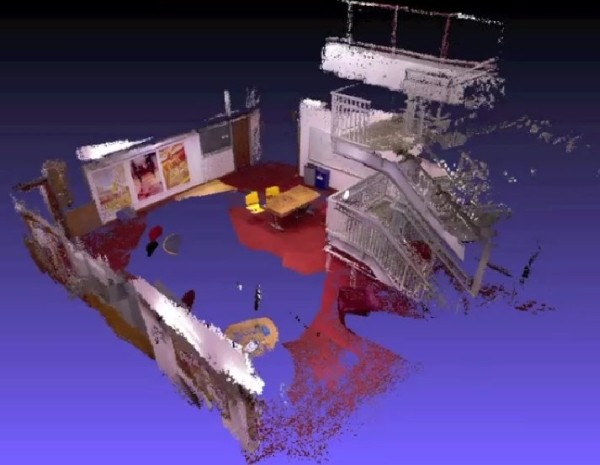
\includegraphics[height=40mm]{kinectslam.jpg}}
  \hspace{5mm}
  \subfloat[Quadrotor helicopter with the Kinect mounted on top.]{\label{fig:kinectquadrotor}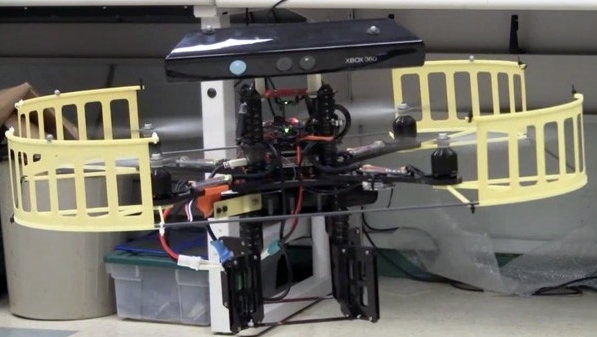
\includegraphics[height=40mm]{kinectquadrotor.jpg}}
  \caption{Kinect projects examples}
  \label{fig:kinectprojects}
	\end{figure}
 
%|-----------------------------------------|
%|--------------- ICUB PART ---------------|
%|-----------------------------------------|

\section{iCub} %\ref{sect:iCub}

The interfaces developed throughout this work have been thought of with the iCub robot in mind. The iCub is an humanoid child robot, spread in several laboratories around the world, being associated with works in fields that go from Electronics and Computer Science to Neuropsychology.

The hardware and software developed within the iCub project is all open source, which makes all the development of the iCub available to anyone interested. This software can be all downloaded form the iCub website\footnote{\url{http://www.robotcub.org/}} \cite{icub:Metta:2008:IHR:1774674.1774683}.

The two following sections are a broad description of the iCub and its programming framework, this introduction was mainly based on two works \cite{icub:Metta:2008:IHR:1774674.1774683} and \cite{icub:5650851}.

\subsection{iCub Robot}

	The iCub is a 140cm tall child, that is able to crawl, sit, and do sophisticated manipulation with its hands, the physical aspect of the robot can be seen in the figure \ref{fig:icubrobot}. The iCub has 53 \ac{DOF}, 39 \ac{DOF} that are distributed through the upper part of the robot body, and 14 \ac{DOF} are in the low part. The hands alone, which are used for manipulation, have 9 \ac{DOF}, with three independent fingers plus other two connected to a single motor. The legs, although not programmed to do that, have enough strength to support the robot on bipedal mode. There is also a set of sensors distributed along the body: cameras, gyroscopes, accelerometers, microphones, and force/torque sensors. A sensitive skin has been developed, but is not yet available at the Instituto de Sistemas e Rob�tica, at the moment this dissertation is being written. With the skin it is possible to detect pressure on the robot outer part, making it possible to grasp objects more precisely, and to control the robot by pushing its parts.
 
 	\begin{figure}[htb]
	\begin{center}
	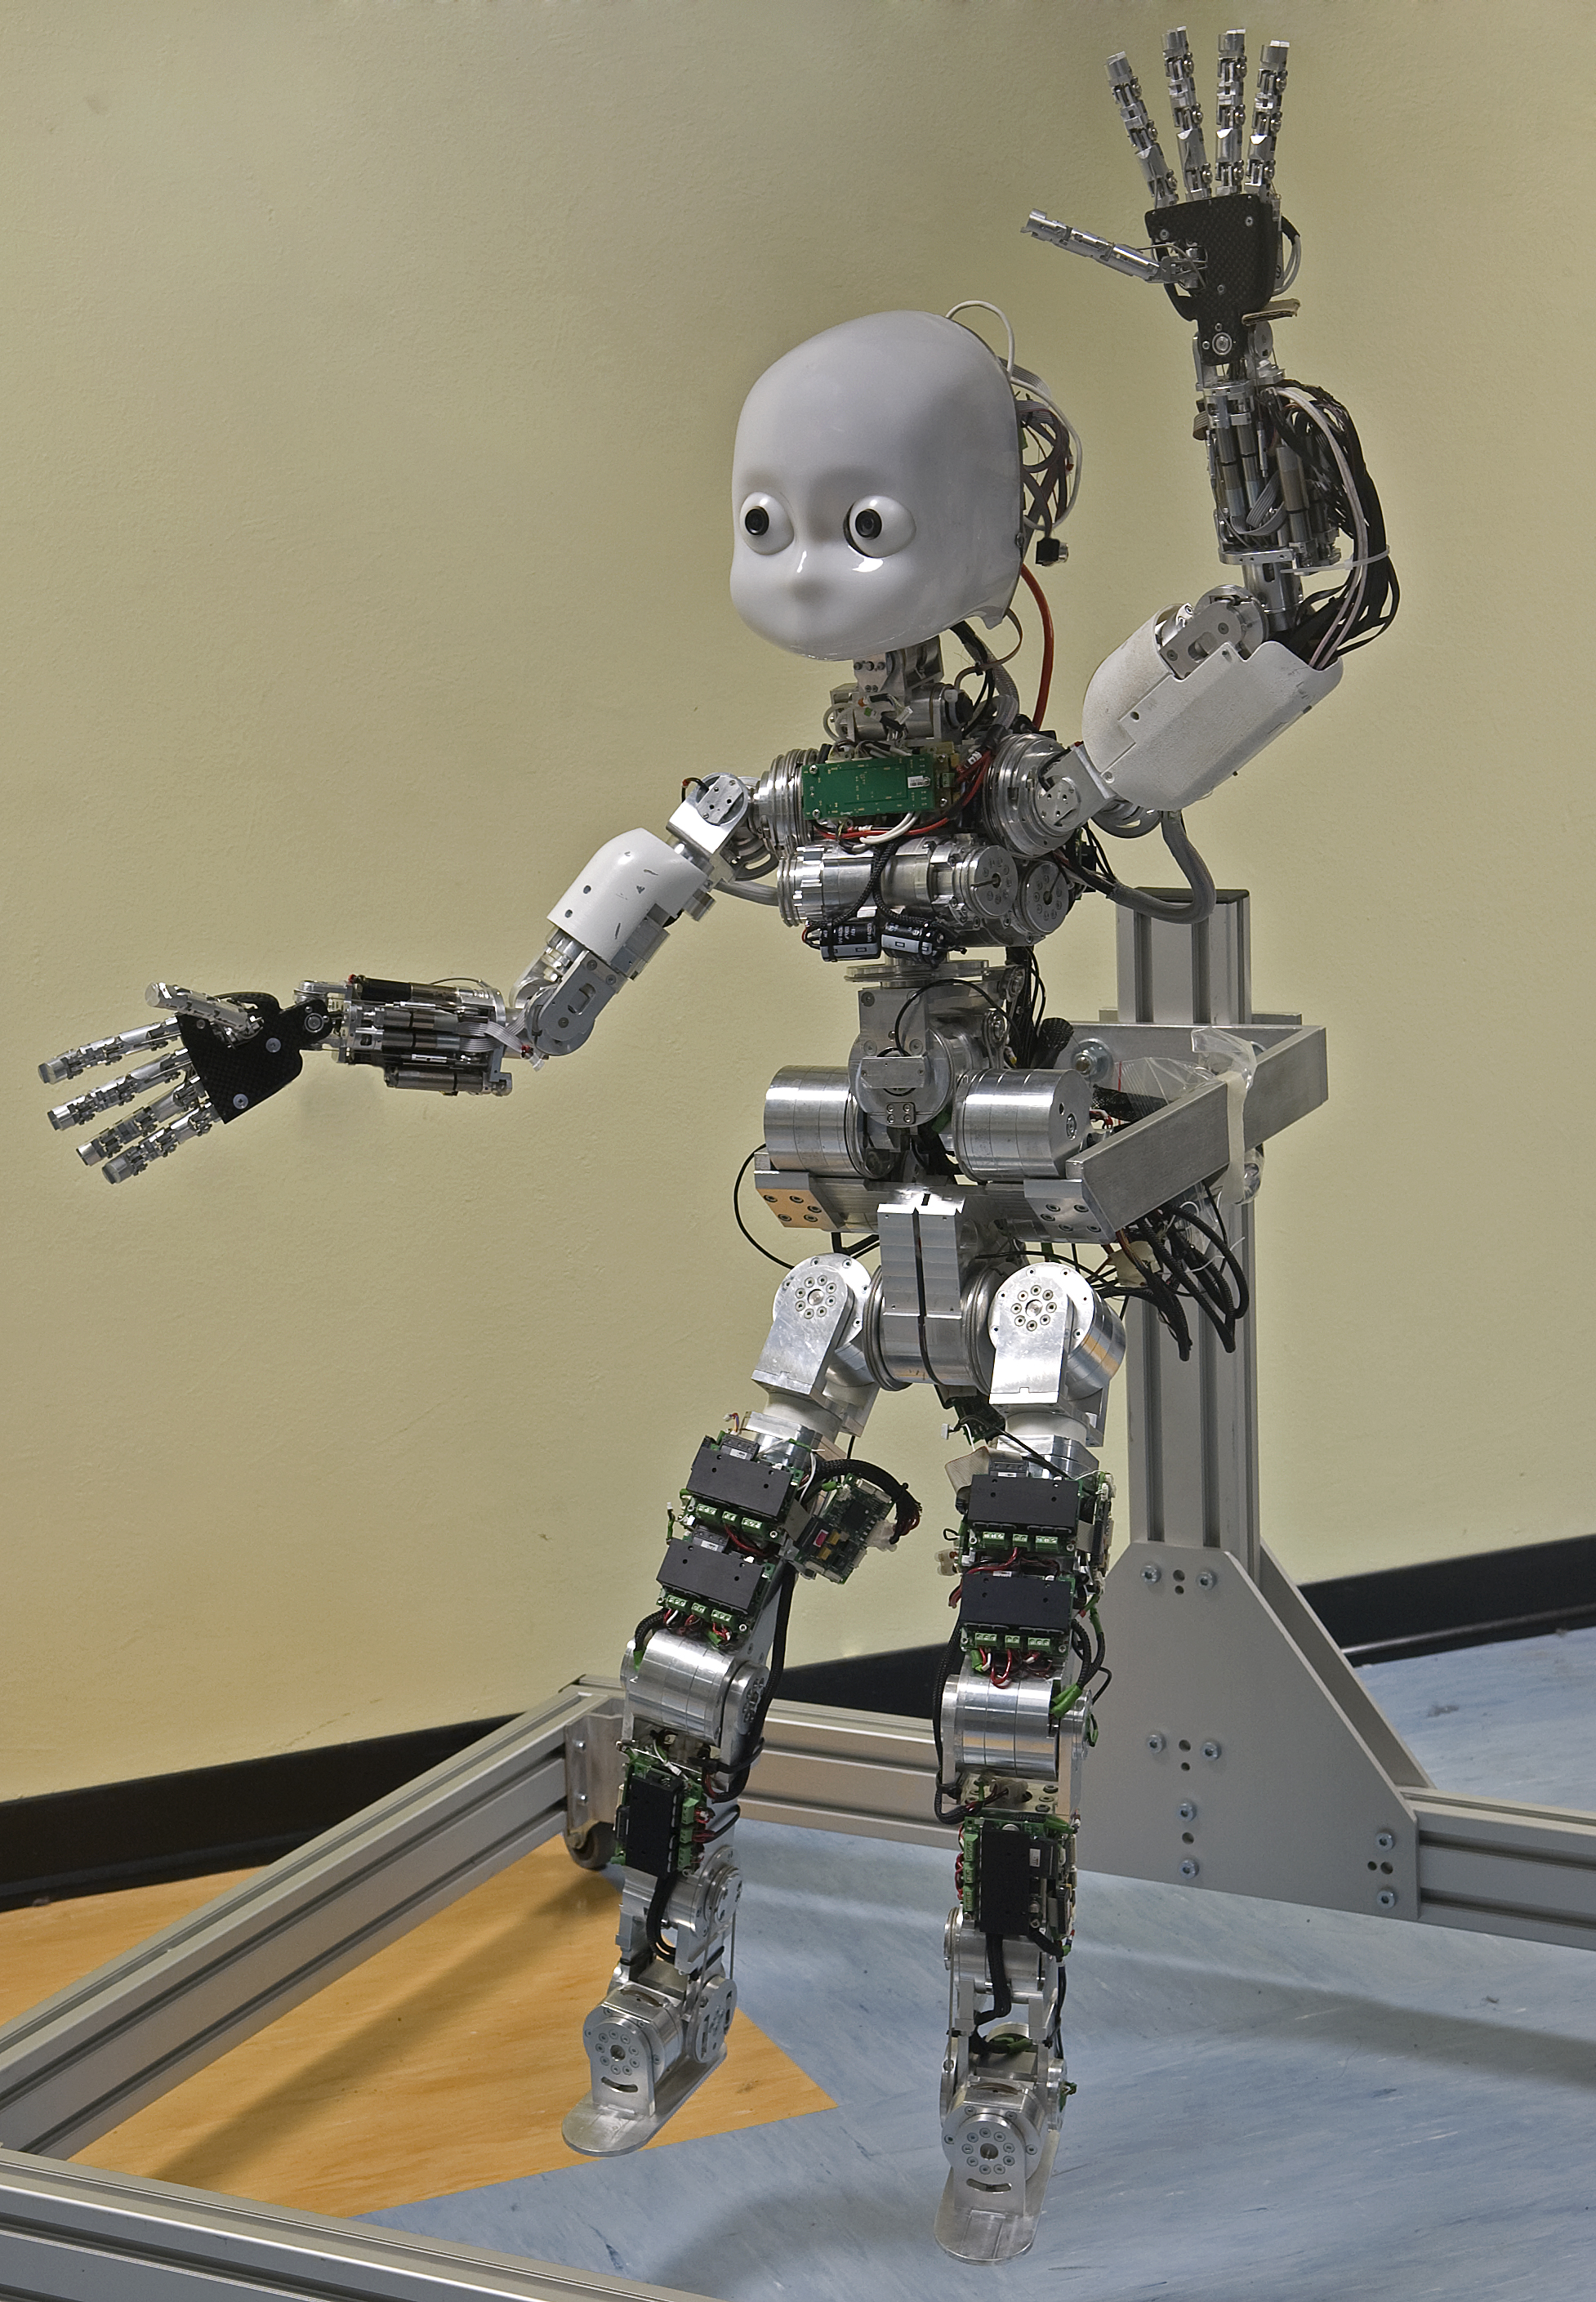
\includegraphics[height=72mm]{icubrobot.jpg}
	\end{center}
	\caption[iCub robot]{iCub robot.} 
	\label{fig:icubrobot}
	\end{figure}

	All the low level control is made through a set of \ac{DSP} based cards, connected via \ac{CAN} bus, specifically designed for the iCub robot. The sensor and motor-state data is passed on to the PC104 card located in the head of the robot, where all that data is reformatted and synchronized with data streams to a Gbit Ethernet connection. Typically the heavier computation is made on independent machines external to the iCub, connect through the iCub Ethernet connection.

	The iCub robot was developed with the goal of: creating an open hardware/software humanoid robotic platform for research in embody cognition, and advancing our understanding of natural and artificial cognitive systems by exploiting this platform in the study of the development of cognitive capabilities \cite{icub:Metta:2008:IHR:1774674.1774683}.
	
	The software and libraries that are available in the iCub open-source repository, allow the development of software for the iCub control. The control of the robot is made through Yarp server, and there is already implemented a inverse kinematic control \cite{icub:5650851} that allows to control the iCub full arm and torso by specifying where should a end-effector reach, typically the robot hand, but any end-effector can be defined.

\subsection{\acf{Yarp}}

	The computation made in independent machines, and in the pc104 inside the iCub robot, uses a framework called \ac{Yarp}. This framework abstracts two common  difficulties in robotics: modularity in algorithms and interfacing with the hardware. \ac{Yarp} is not iCub specific, what obliges the iCub to have some specific software written to be able to take care of the abstraction between the iCub and the framework and prepare the robot to receive \ac{Yarp}-like instructions.

	The main abstractions of \ac{Yarp} are the \textit{ports}. \textit{Ports} implement the observer pattern that allows to send a message through one port, to a multiple number of ports that are distributed across different computers, this way the sender and receiver can work independently. The observer pattern is a broadly used software design pattern where an object, the subject, maintains a list of its dependents, the observers, the observers are notified each time that the subject considers it necessary. The subject in ports would be a writer port, and the observers would be read ports that are connected to the subject port.
	
	Another abstraction implemented by \ac{Yarp} is the \textit{device}, that allows to specify which device the programmer/user wants to interact with and the framework provides an object that hides the low-level programming details. This pair of \textit{port}/\textit{device} allows for the development of a remote device driver that can be used across a network, making the heavier processing independent from the robot hardware.

	The \ac{Yarp} framework divides the default \textit{devices} into many abstractions that can be used, such as IPositionControl, IVelocityControl or IKin. Those abstractions are used to control the robot mechanics and sensors without having to be worried with the low-level instructions. \ac{Yarp} does this by providing an object with simple control functions such as the \texttt{positionMove()}, \texttt{velocityMove()}, or \texttt{setRefSpeeds()}. Some of these device objects need exterior modules to be running to support all of the actions available. Typically what these device objects do is no more than creating \textit{ports}, to send and receive messages to the control boards of the robot or to external modules that do other work.

\section{Concluding remarks}

	In this chapter were presented the several elements of the work to be developed: \ac{HRI}, the interaction devices \ac{Wiimote} and Kinect sensor, the iCub robot, and the \ac{Yarp} framework.
	
	Due to the lack of autonomy that still exists in robots today, \ac{HRI} is still very focused in controlling robots through several ways, such as teleoperation to achieve a natural and intuitive interaction, in a natural and intuitive way.
	
	The gaming industry has been developing several user interface devices, that are meant for games control, but that offer very high technology solutions that  can be adapted to the robot interfaces challenges, and have as advantages robustness and low price. The \ac{Wiimote} and Kinect are two of the latest devices that have been made available, and they are being adapted for a wide range of interaction projects from art to robotics with very interesting results.
	
	In this work case the iCub robot will be used for the development of interfaces that save developers time, and allow for easy interaction with first time users is a good application for the cognitive study and interactive learning. Some of the most sophisticated robots available are used as helpers that need constant control for very specific tasks, but the control form should be simplified and use metaphors that are understood by users, this new interfaces allow for new metaphors to be created.
	
	To interface with the systems and devices \ac{Yarp} will be used, which allows for a easy separation of the logic blocks of our application.
	
	There are not many projects released using robotics and the Kinect or \ac{Wiimote}/\ac{MP} but it is certain that this is a mixture that is going to be appearing in many other works in the near future adapted to many different tasks in robotics.